\section{A Rule-Based Reachability Criterion}

\sepfootnotecontent{sf:opensSource}{
The implementation, the queries and the evaluation are available at the following links:\newline
\href{https://github.com/constraintAutomaton/comunica-feature-link-traversal/tree/feature/time-filtering-tree-sparqlee-implementation}{https://github.com/constraintAutomaton/comunica-feature-link-traversal/tree/feature/time-filtering-tree-sparqlee-implementation},
\href{https://github.com/TREEcg/TREE-Guided-Link-Traversal-Query-Processing-Evaluation/tree/main}{https://github.com/TREEcg/TREE-Guided-Link-Traversal-Query-Processing-Evaluation/tree/main}
}

\sepfootnotecontent{sf:predicateCriterion}{
The query engine will always follow \texttt{ex:nextNode} from expressions following the schema "\texttt{ex:currentNode tree:relation [tree:node ex:nextNode]}" regardless of the constraints.
}

\sepfootnotecontent{sf:reachabilityCriterion}{
    We use a simplified formalization to illustrate the source selection mechanism and to not introduce unnecessary concepts for the aim of this poster paper. 
}

Most research on LTQP is centered around query execution in Linked Open Data environments.
Given the pseudo-infinite number of documents on the Web, traversing over all documents is practically infeasible.
To define completeness, different reachability criteria~\cite{hartig2012} were introduced to allow the discrimination of links.
Recently, an alternative direction was designed where the query engine uses the structure from the data publisher to guide itself towards relevant data sources~\cite{taelman2023, verborgh2020}.

We define our approach as a rule-based reachability criterion.
Our approach builds upon the concept of structural assumptions~\cite{taelman2023} to exploit the structural properties of TREE annotated datasets.
We therefore interpret the hypermedia descriptions of constraints in TREE fragments as boolean expressions $E$ ($?t>= \text{2022-01-03T09:47:59.000000}$ in Figure~\ref{lst:system}).
Upon discovery of a document, the query engine gathers the relevant triples to form the boolean expression of the constraint on the data of reachable fragments.
After the parsing of the expression, the filter expression $F$ of the SPARQL query is \textit{pushed down} into the engine's source selection component.
The source selection component can be formalized as a reachability criterion~\sepfootnote{sf:reachabilityCriterion} 
\begin{equation}
c(i) \rightarrow \{\mathrm{true}, \mathrm{false}\}
\end{equation}
where when it returns $\mathrm{true}$ the target IRI $i$ \emph{must} be dereferenced.
Finally, the two boolean expressions are evaluated to determine their satisfiability.
It can be formalized as determining if 
\begin{equation}
    c(i) = \exists x | (F(x) \land E_i) = \mathrm{true}
\end{equation}
hold true given $x$ is the variable targeted by $E_i$ and $i$ is the link towards the next fragment (\texttt{<nextNode>} from ``\texttt{<> tree:node <nextNode>}'' in Figure~\ref{lst:system}).
A variable targetted by $E$ is defined by an RDF object where the predicate as a value \texttt{?target} from the triple
defining the fragmentation path in the form ``''\texttt{?s tree:path ?target}'' (\texttt{saref:hasTimestamp} in Figure~\ref{lst:system}).
Upon satisfaction the IRI targeting the next fragment is added to the link queue otherwise the IRI is pruned.
The process is schematized in Figure~\ref{fig:process}.

\begin{figure}[htbp]
    \centering
    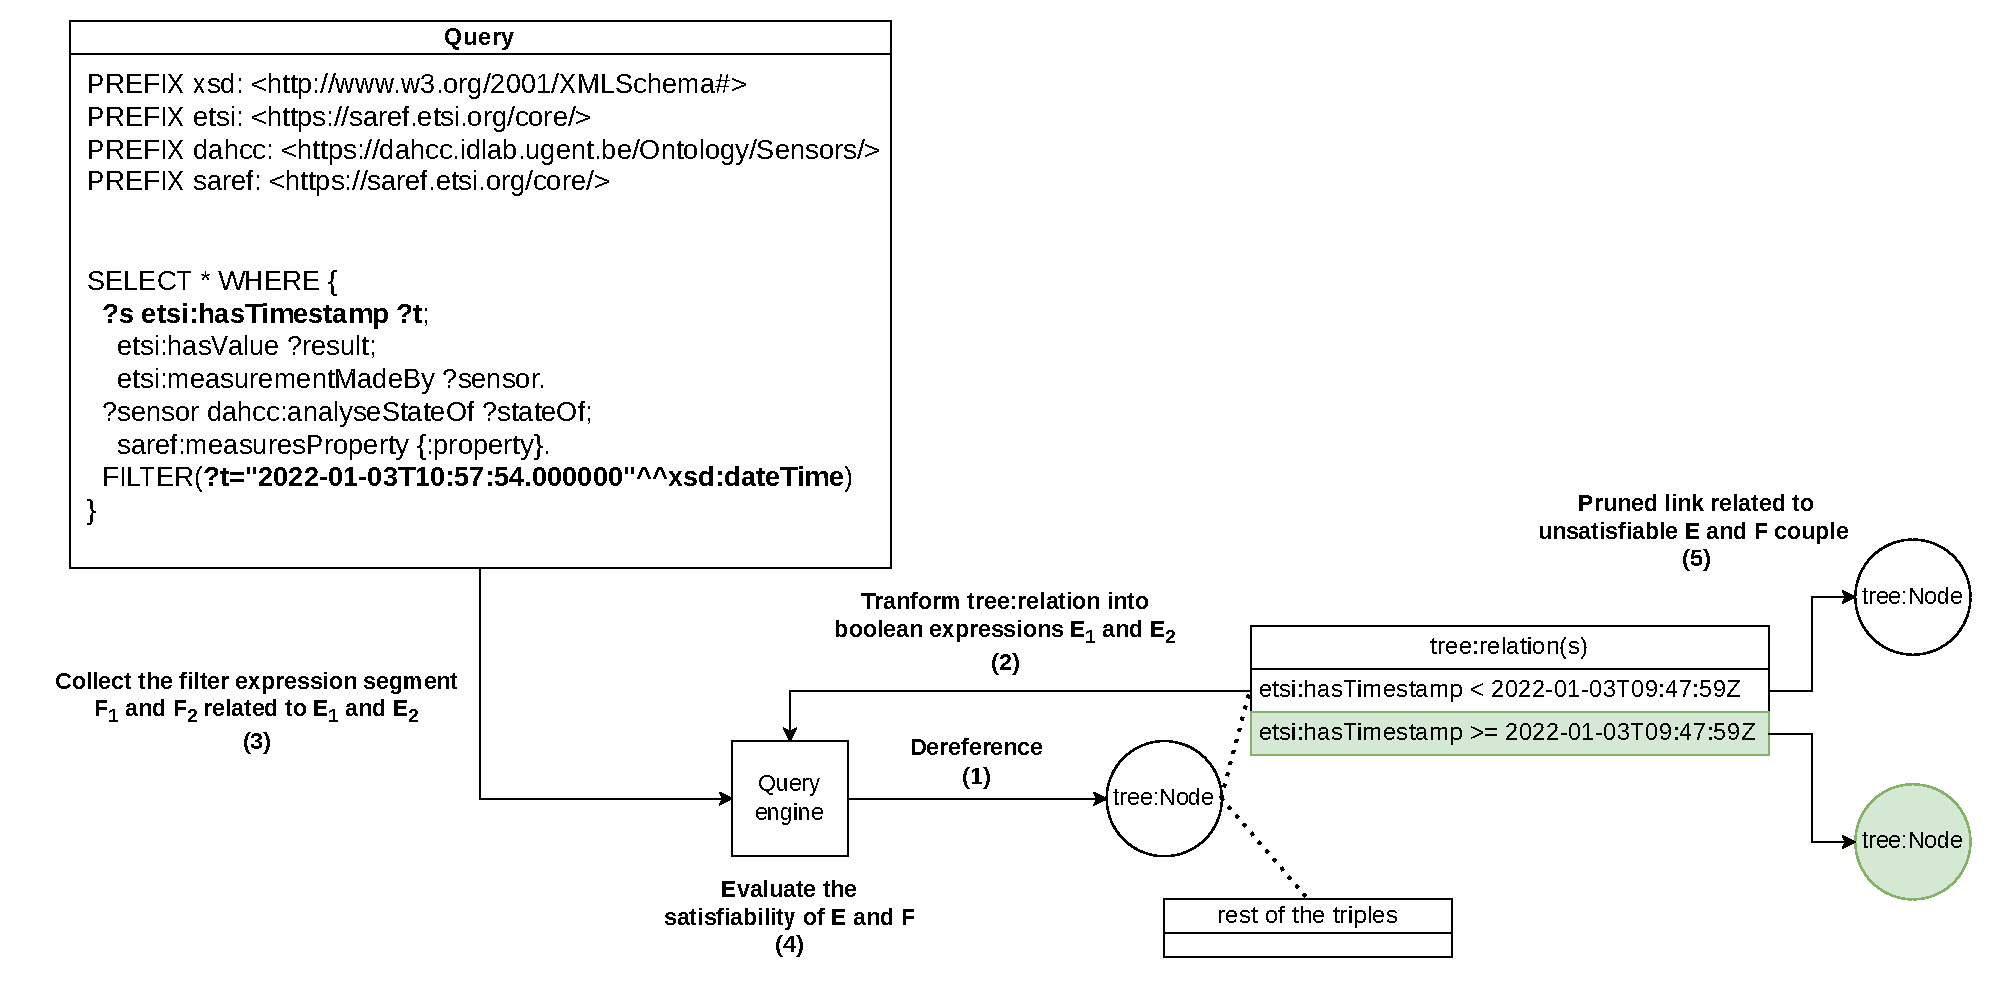
\includegraphics[width=\linewidth]{image/running_example.drawio.pdf}
    \caption{A schematization of our rule-based reachability criteria with a TREE document.
      First a TREE node is dereferenced, then the TREE relations are transformed into boolean expressions $E$,
      followed by the construction of $F$ from the filter expression related to the path of $E$ (the variable $t$ related to \texttt{saref:hasTimestamp}),
       then the satisfiability $E \land F$ is determined and finally links to non-query relevant data are pruned.}
    \label{fig:process}
  \end{figure}

\subsection{Preliminary Results}

We implemented our approach using the query engine Comunica~\cite{comunica}.
For evaluation, we executed four queries similar to the one in Figure \ref{lst:system}.~\sepfootnote{sf:opensSource}
They were executed over the DAHCC participant 31 dataset~\cite{dahcc_resource} (487 MB) with a timeout of two minutes.
We fragmented the dataset according to the TREE specification.
We use a B-tree topology with a depth of 1 using 100 and 1000 nodes ($n$).

\begin{table}[ht]
    \centering
    \begin{tabular}{|c|c|c|c|c|c|}
        \hline
        \textbf{n} & \textbf{Query} & \textbf{Time-predicate (ms)}  & \textbf{Time-rule (ms)} & \textbf{HTTP-request-rule} & \textbf{Res-rule} \\
        \hline
        100 & Q1 & x & 8,892& 3 & 0 \\
        100 & Q2 & x & 3,541& 3 & 1 \\
        100 & Q3 & x & 59,274& 8 & 8,166 \\
        \hhline{|=|=|=|=|=|=|}
        1000 & Q1 & x & 1,171& 3 & 0 \\
        1000 & Q2 & x & 734& 3 & 1 \\
        1000 & Q3 & x & 39,987& 51 & 8,166 \\
        \hline
    \end{tabular}
    \caption{
    The predicate-based (-predicate) reachability criterion is not able to execute the queries. 
    The rule-based (-rule) criterion performs better in term of execution time (Time) with a larger number of fragments even when performing more HTTP requests (HTTP-request).
    Q4 is not depicted because the instances were not able to terminate before the timeout.
    }
    \label{tab:result}
    \vspace*{-0.15cm}
\end{table}

The queries were executed using two configurations.
In the first configuration, we use a predicate-based reachability criterion where the engine follows each link of the fragmented dataset.~\sepfootnote{sf:predicateCriterion}
For the second one, we use our rule-based reachability criterion approach.
As shown in Table \ref{tab:result} no queries could be answered within the timeout by following every fragment.
A possible explanation is the high number of HTTP requests performed~\cite{Hartig2016} leading to non-relevant data sources. 
With our rule-based reachability criterion, the queries executed over the 1000 nodes fragmentation perform better than the ones with 100 nodes.
The query execution time has a percentage of reduction of 86\% with Q1 and 79\% with Q2 compared to the fragmentation with 100 nodes.
With Q3 we see that the percentage of reduction is 33\%, this lowering of performance gain might be caused by the increase by a factor of 6 in HTTP requests.
This raises an interesting observation because we do not observe a reduction in execution time with a reduction in HTTP requests.
Previous research has proposed that inefficient query plans might be the bottleneck of some queries in structured environments~\cite{taelman2023,eschauzier_quweda_2023}.
However, our results seem to show that the size of the internal triple store might have a bigger impact on performance than noted in previous studies.
As large-scale link traversal over the web will result in the acquisition of a large number of triples, a future interesting research direction would be to find ways to remove triples that are certain to not lead to a query result from the internal triple store.
The query Q4 was not able to be answered, with any setup, because the query requires a larger number of fragments than the other to be processed.
